39. $\cfrac{x^2-y^2}{x^2+y^2-9}=0\Leftrightarrow \begin{cases} x^2-y^2=0,\\ x^2+y^2-9\neq0\end{cases}
\Leftrightarrow \begin{cases}\left[\begin{array}{l} y=x,\\ y=-x.\end{array}\right.\\ x^2+y^2\neq3^2\end{cases}$
$$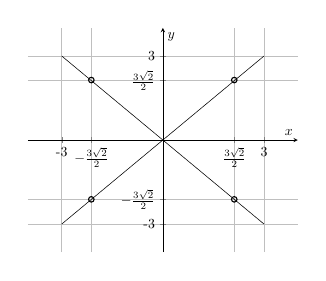
\begin{tikzpicture}[scale=0.5]
\begin{axis}[
    axis lines = middle,
    grid=major,
    legend pos={south west},
    xlabel = {$x$},
    %xlabel style={below right},
    ylabel = {$y$},
    ymin=-4,
    ymax=4,
    xmin=-4,
    xmax=4,
    xtick={-3,-2.12,2.12,3},
    xticklabels={-3,$-\frac{3\sqrt{2}}{2}$,$\frac{3\sqrt{2}}{2}$,3},
    ytick={-3,-2.12,2.12,3},
    yticklabels={-3,$-\frac{3\sqrt{2}}{2}$,$\frac{3\sqrt{2}}{2}$,3},
                  ]
	\addplot[domain=-3:3, samples=100, color=black] {x};
    \addplot[domain=-3:3, samples=100, color=black] {-x};
     %\addlegendentry{$\text{Рис. 1}$};
\end{axis}
\draw (5.24,4.37) circle (2pt);
\draw (1.61,4.37) circle (2pt);
\draw (1.61,1.34) circle (2pt);
\draw (5.24,1.34) circle (2pt);
\end{tikzpicture}$$
